\documentclass[aspectratio=169,11pt]{beamer}

% ---------- Academic Beamer style ----------
\usetheme{Boadilla}
\usefonttheme{professionalfonts}
\setbeamertemplate{navigation symbols}{}
\setbeamertemplate{blocks}[rounded][shadow=false]
\setbeamertemplate{itemize items}[circle]
\setbeamertemplate{enumerate items}[default]

\usepackage[T1]{fontenc}
\usepackage{lmodern}
\usepackage{amsmath,amssymb,mathtools}
\usepackage{booktabs,tabularx,array}
\usepackage{tikz}
\usetikzlibrary{arrows.meta,positioning,shapes.geometric,calc}
\usepackage{hyperref}

\definecolor{Navy}{HTML}{17324D}
\definecolor{Teal}{HTML}{087E83}
\definecolor{PaleTeal}{HTML}{EAF4F4}
\definecolor{Slate}{HTML}{455564}
\definecolor{LightLine}{HTML}{D8E1E8}
\definecolor{Gold}{HTML}{C59A3D}

\setbeamercolor{structure}{fg=Teal}
\setbeamercolor{palette primary}{bg=Navy,fg=white}
\setbeamercolor{palette secondary}{bg=Navy!90,fg=white}
\setbeamercolor{palette tertiary}{bg=Navy!80,fg=white}
\setbeamercolor{palette quaternary}{bg=Navy,fg=white}
\setbeamercolor{frametitle}{fg=Navy,bg=white}
\setbeamercolor{title}{fg=Navy}
\setbeamercolor{subtitle}{fg=Slate}
\setbeamercolor{block title}{fg=white,bg=Navy}
\setbeamercolor{block body}{fg=Slate,bg=Navy!4}
\setbeamercolor{alerted text}{fg=Teal}
\setbeamercolor{normal text}{fg=Slate,bg=white}
\setbeamercolor{author in head/foot}{fg=white,bg=Navy!82}
\setbeamercolor{date in head/foot}{fg=white,bg=Navy}

\setbeamerfont{title}{size=\LARGE,series=\bfseries}
\setbeamerfont{subtitle}{size=\large}
\setbeamerfont{frametitle}{size=\Large,series=\bfseries}
\setbeamerfont{footline}{size=\scriptsize}
\setbeamertemplate{frametitle}{%
  \vspace{0.15em}%
  \begin{beamercolorbox}[wd=\paperwidth,ht=3.2ex,dp=1.15ex,leftskip=0.55cm,rightskip=0.4cm]{frametitle}%
    \insertframetitle\hfill{\color{Teal}\rule{0pt}{1.2ex}}%
  \end{beamercolorbox}%
  \vspace{-0.3em}\hspace{0.55cm}{\color{Teal}\rule{0.9cm}{1.4pt}}%
  \vspace{0.25em}%
}
\setbeamertemplate{footline}{%
  \leavevmode%
  \hbox{%
    \begin{beamercolorbox}[wd=.84\paperwidth,ht=2.7ex,dp=1.1ex,leftskip=0.55cm]{author in head/foot}%
      \color{white}\insertshorttitle
    \end{beamercolorbox}%
    \begin{beamercolorbox}[wd=.16\paperwidth,ht=2.7ex,dp=1.1ex,rightskip=0.55cm plus 1fil]{date in head/foot}%
    \hspace{0.5cm}\color{white}\insertframenumber\,/\,13
    \end{beamercolorbox}%
  }%
  \vskip0pt%
  \color{Teal}\rule{\paperwidth}{0.7pt}%
}

\newcommand{\source}[1]{\par\vspace{-0.15cm}\hfill{\fontsize{4.5}{5.2}\selectfont\color{Slate!65}Source: NIST FIPS 203, #1.}}
\newcommand{\Rq}{\mathcal{R}_q}
\newcommand{\KEM}{\textsc{ML-KEM}}
\newcommand{\PKE}{\textsc{K-PKE}}
\newcommand{\B}{\{0,1\}}

\title[FIPS 203: ML-KEM]{FIPS 203: Module-Lattice-Based Key-Encapsulation Mechanism}
\author{Sarbo Sarcar, Daniyal Anis, Srijani Roy}
\institute{Department of Information Technology, Jadavpur University}
\date{}

\begin{document}

% ---------- Slide 1: Title ----------

\begin{frame}[plain]

    % Left-aligned content block
    \vspace*{1.25cm}
    \hspace*{1.05cm}
    \begin{minipage}{0.78\textwidth}

        % Main title
        {\fontsize{20}{34}\selectfont
        \bfseries\color{Navy} FIPS 203\par}

        \vspace{0.18cm}

        % Subtitle
        {\fontsize{14}{21}\selectfont
        \bfseries\color{Navy}
        Module-Lattice-Based\\[-1pt]
        Key-Encapsulation Mechanism\par}

        \vspace{0.22cm}

        % Decorative line
        {\color{Teal}\rule{2.2cm}{1.3pt}\par}

        \vspace{0.48cm}

        % Authors and affiliation
        {\small
        Sarbo Sarcar (002311001011)\par
        \vspace{0.07cm}
        Daniyal Anis (002311001022)\par
        \vspace{0.07cm}
        Srijani Roy (002311001026)\par
        }

        \vspace{0.06cm}

        {\small
        4$^\text{th}$ Year 1$^\text{st}$ Semester\par
        Dept. of Information Technology\par
        Jadavpur University\par
        }

    \end{minipage}

    \vfill

\end{frame}


% ---------- Slide 2: Agenda ----------
\begin{frame}{Agenda}
  \begin{enumerate}
    \setlength{\itemsep}{0.62em}
    \item Post-quantum motivation and purpose of FIPS 203
    \item Module Learning With Errors (MLWE): mathematical foundation
    \item ML-KEM key generation
    \item Encapsulation: deriving a shared secret and ciphertext
    \item Decapsulation: verification and implicit rejection
    \item Parameter sets and practical implementation components
  \end{enumerate}
  % \source{Sections 1, 3--8}
\end{frame}

% ---------- Slide 3: Motivation and standard ----------
\begin{frame}{Why PQC? What FIPS 203 Specifies}
  \begin{columns}[T,onlytextwidth]
    \column{0.49\textwidth}
      \begin{block}{The motivation}
        \footnotesize
        \begin{itemize}
          \setlength{\itemsep}{0.15em}
          \item RSA %(Rivest--Shamir--Adleman) 
          relies on integer factorisation; %DH 
          Diffie--Hellman and ECC %(elliptic-curve cryptography) 
          rely on discrete logarithms.
          \item Shor's algorithm threatens both assumptions on a sufficiently capable fault-tolerant quantum computer.
          \item PQC (post-quantum cryptography) develops schemes intended to resist known classical and quantum attacks.
        \end{itemize}
      \end{block}
    \column{0.49\textwidth}
      \begin{block}{The FIPS 203 standard}
        \footnotesize
        \begin{itemize}
          \setlength{\itemsep}{0.15em}
          \item NIST (National Institute of Standards and Technology) 
          published FIPS (Federal Information Processing Standards) 
          203 on 13 August 2024.
          \item It specifies ML-KEM (Module-Lattice-Based Key-Encapsulation Mechanism), a KEM (key-encapsulation mechanism) based on Module-LWE (Module Learning With Errors).
          \item It establishes a shared 256-bit secret; symmetric cryptography then uses that secret.
        \end{itemize}
      \end{block}
  \end{columns}
  \vspace{0.02cm}
  \begin{beamercolorbox}[rounded=true,sep=0.30em,wd=\linewidth,center]{block body}
    \scriptsize
    \textbf{KEM interface:}\quad
    $(ek,dk)\leftarrow\operatorname{KeyGen}()$;\quad
    $(K,c)\leftarrow\operatorname{Encaps}(ek)$;\quad
    $K'\leftarrow\operatorname{Decaps}(dk,c)$.\\[1pt]
    $ek$: public encapsulation key; $dk$: private decapsulation key; valid ciphertext: $K'=K$.
  \end{beamercolorbox}
  \source{Sections 1 and 3.1--3.2}
\end{frame}

% ---------- Slide 4: MLWE ----------
\begin{frame}{Mathematical Foundation: Module Learning With Errors}
  \small
  \begin{block}{Polynomial ring used by ML-KEM}
    \[
      \mathcal{R}_q=\mathbb{Z}_q[X]/(X^n+1),\qquad
      \mathbb{Z}_q=\mathbb{Z}/q\mathbb{Z},\quad n=256,\quad q=3329.
    \]
    Each polynomial has degree below $n$; its coefficients are reduced modulo $q$, and $X^n\equiv-1$.
  \end{block}
  \vspace{0.03cm}
  \begin{center}
    \fbox{\large $\displaystyle t=A s+e\quad\text{over }\mathcal{R}_q$}
  \end{center}
  \vspace{0.02cm}
  \begin{columns}[T,onlytextwidth]
    \column{0.52\textwidth}
      \begin{itemize}
        \setlength{\itemsep}{0.17em}
        \item $A\in\mathcal{R}_q^{k\times k}$: public matrix
        \item $s,e,t\in\mathcal{R}_q^k$: secret, noise, and public vectors
        \item $k$ is the module dimension; for ML-KEM-768, $k=3$.
        \item $e$ is sampled from a small centred-binomial distribution.
      \end{itemize}
    \column{0.44\textwidth}
      \begin{alertblock}{Why Module-LWE matters}
        The public pair $(A,t)$ gives noisy polynomial equations. Recovering $s$ from $(A,t)$ is presumed computationally hard for the approved parameters, including for quantum adversaries.
      \end{alertblock}
  \end{columns}
  \source{Sections 2, 3.2, and 4}
\end{frame}

% ---------- Slide 5: Key Generation ----------
\begin{frame}{ML-KEM Key Generation}
  \small
  \textbf{Goal:} generate public encapsulation key $ek$ and private decapsulation key $dk$.\par\vspace{0.10cm}
  \begin{columns}[T,onlytextwidth]
    \column{0.57\textwidth}
      \footnotesize
      \begin{enumerate}
        \setlength{\itemsep}{0.08em}
        \item Sample independent 32-byte seeds $d,z$ using an approved random bit generator (RBG).
        \item Expand the seeds using the one-byte encoding of $k$:
          \[
            (\rho,\sigma)=G(d\parallel\operatorname{byte}(k)).
          \]
        \item Use $\rho$ to expand $\widehat A$; use $\sigma$ to sample small vectors $s,e$. Compute:
          \[
            \widehat s=\operatorname{NTT}(s),\quad
            \widehat e=\operatorname{NTT}(e),\quad
            \widehat t=\widehat A\circ\widehat s+\widehat e.
          \]
        \item Encode the keys:
          \[
            \begin{aligned}
              ek&=\operatorname{ByteEncode}_{12}(\widehat t)\parallel\rho,\\[-1pt]
              dk&=\operatorname{ByteEncode}_{12}(\widehat s)\parallel ek\parallel H(ek)\parallel z.
            \end{aligned}
          \]
      \end{enumerate}
    \column{0.40\textwidth}
      \begin{alertblock}{What do $\rho$ and $\sigma$ mean?}
        \footnotesize
        \begin{itemize}
          \setlength{\itemsep}{0.22em}
          \item $\rho$: public 32-byte seed appended to $ek$ and used to regenerate $\widehat A$.
          \item $\sigma$: 32-byte seed expanded to sample the secret vector $s$ and error vector $e$.
        \end{itemize}
      \end{alertblock}
      \vspace{0.02cm}
      \begin{beamercolorbox}[rounded=true,sep=0.38em,wd=\linewidth]{block body}
        \scriptsize
        NTT: Number-Theoretic Transform; $\widehat{\;}$ denotes the NTT representation; $\circ$ is pointwise multiplication; $\parallel$ denotes byte concatenation.\\[2pt]
        $H=\mathrm{SHA3\mbox{-}256}$; $G=\mathrm{SHA3\mbox{-}512}$.
      \end{beamercolorbox}
  \end{columns}
  \source{Sections 4.1, 4.3, 5.1, 6.1, and 7.1}
\end{frame}

% ---------- Slide: K-PKE Internal Architecture ----------
\begin{frame}{Under the Hood: The Internal $\PKE$ Scheme}
  \small
  $\KEM$ wraps an underlying IND-CPA secure public-key encryption scheme ($\PKE$):
  \vspace{0.15cm}
  \begin{columns}[T,onlytextwidth]
    \column{0.49\textwidth}
      \begin{block}{$\PKE.\mathrm{Encrypt}(ek, m, r)$}
        \footnotesize
        \begin{enumerate}
          \setlength{\itemsep}{0.25em}
          \item Regenerate $\widehat A$ from seed $\rho$; sample small noise vectors $r, e_1 \in \mathcal{R}_q^k$ and $e_2 \in \mathcal{R}_q$.
          \item Encode message $m \in \{0,1\}^{256}$ as polynomial $\mu \in \mathcal{R}_q$ (coefficients in $\{0, \lceil q/2 \rfloor\}$).
          \item Compute noisy ciphertext components:
            \[
              u = A^T r + e_1, \qquad v = t^T r + e_2 + \mu
            \]
          \item Return $c = (\operatorname{Compress}_{d_u}(u), \operatorname{Compress}_{d_v}(v))$.
        \end{enumerate}
      \end{block}

    \column{0.49\textwidth}
      \begin{block}{$\PKE.\mathrm{Decrypt}(dk_{\PKE}, c)$}
        \footnotesize
        \begin{enumerate}
          \setlength{\itemsep}{0.25em}
          \item Decompress $u$ and $v$ to recover $\tilde{u}, \tilde{v} \in \mathcal{R}_q$.
          \item Compute noisy message polynomial:
            \[
              w = \tilde{v} - s^T \tilde{u} \approx \mu + \text{noise}
            \]
          \item Decode coefficients: round each coefficient near $\lceil q/2 \rfloor$ to $1$, near $0$ to $0$.
          \item Return reconstructed 32-byte message $m'$.
        \end{enumerate}
      \end{block}
  \end{columns}
  \source{Section 5}
\end{frame}

% ---------- Slide 6: Encapsulation flow ----------
\begin{frame}{Encapsulation: Generate the Shared Secret}
  \begin{columns}[T,onlytextwidth]
    \column{0.47\textwidth}
      \begin{block}{Inputs and computation}
        \small
        \begin{enumerate}
          \setlength{\itemsep}{0.26em}
          \item Input: checked public encapsulation key $ek$.
          \item Sample fresh random $m\in\{0,1\}^{256}$ (32 bytes).
          \item Derive $(K,r)=G(m\parallel H(ek))$; $r$ is the encryption randomness.
          \item Compute $c=\PKE.\mathrm{Encrypt}(ek,m,r)$.
        \end{enumerate}
      \end{block}
      \footnotesize\textbf{Output:} $K$ (32 bytes) and ciphertext $c$.
    \column{0.51\textwidth}
      \centering
      \vspace{0.25cm}
      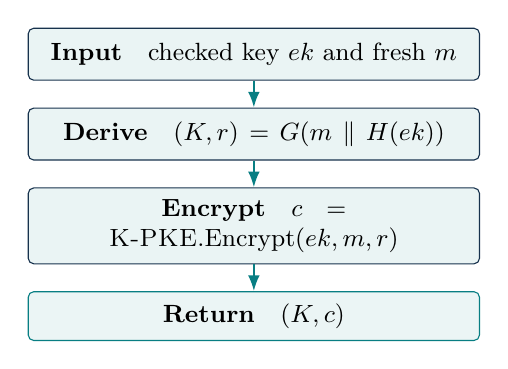
\begin{tikzpicture}[
        node distance=0.34cm,
        flow/.style={draw=Navy,rounded corners=2pt,fill=PaleTeal,align=center,
                     text width=5.45cm,minimum height=0.66cm,font=\small,inner sep=4pt},
        output/.style={draw=Teal,rounded corners=2pt,fill=Teal!8,align=center,
                       text width=5.45cm,minimum height=0.62cm,font=\small,inner sep=4pt},
        arr/.style={-{Latex[length=2mm]},thick,draw=Teal}
      ]
        \node[flow] (input) {\textbf{Input}\quad checked key $ek$ and fresh $m$};
        \node[flow,below=of input] (derive) {\textbf{Derive}\quad $(K,r)=G(m\parallel H(ek))$};
        \node[flow,below=of derive] (encrypt) {\textbf{Encrypt}\quad $c=\PKE.\mathrm{Encrypt}(ek,m,r)$};
        \node[output,below=of encrypt] (result) {\textbf{Return}\quad $(K,c)$};
        \draw[arr] (input) -- (derive);
        \draw[arr] (derive) -- (encrypt);
        \draw[arr] (encrypt) -- (result);
      \end{tikzpicture}
  \end{columns}
  \vspace{0.02cm}
  \begin{center}\scriptsize $\PKE$ is ML-KEM's internal public-key encryption component; it is not a stand-alone scheme. The ciphertext $c$, not $K$, is sent to the decapsulating party.\end{center}
  \source{Sections 4.1, 5.2, 6.2, and 7.2}
\end{frame}

% ---------- Slide 7: Decapsulation in lists and arrowed text ----------
\begin{frame}{Decapsulation: Recover the Shared Secret}
  \small
  \begin{columns}[T,onlytextwidth]
    \column{0.57\textwidth}
      \textbf{Inputs:} checked decapsulation key $dk$ and ciphertext $c$. No fresh randomness is used.
      \vspace{0.10cm}
      \footnotesize
      \begin{enumerate}
        \setlength{\itemsep}{0.17em}
        \item Parse: $dk\mapsto(dk_{\PKE},ek_{\PKE},h,z)$, where $h=H(ek)$ is stored in $dk$.
        \item Decrypt: $m'=\PKE.\mathrm{Decrypt}(dk_{\PKE},c)$.
        \item Derive: $(K',r')=G(m'\parallel h)$.
        \item Re-encrypt: $c'=\PKE.\mathrm{Encrypt}(ek_{\PKE},m',r')$.
      \end{enumerate}
    \column{0.40\textwidth}
      \begin{block}{Implicit rejection}
        \centering
        \footnotesize
        Compute the fallback secret:
        \[
          \overline K=J(z\parallel c).
        \]
        Compare the ciphertexts:
        \[
          K_{\mathrm{out}}=
          \begin{cases}
            K', & c'=c,\\[2pt]
            \overline K, & c'\ne c.
          \end{cases}
        \]
        Return $K_{\mathrm{out}}$ (32 bytes).\\[2pt]
        $J(x)=\mathrm{SHAKE256}(x,256\text{ bits})$.\\[2pt]
        \scriptsize The comparison flag remains secret.
      \end{block}
  \end{columns}
  \vspace{0.06cm}
  \begin{beamercolorbox}[rounded=true,sep=0.30em,wd=\linewidth,center]{block body}
    \scriptsize
    \textbf{Flow:}\quad Parse $dk,c$ $\longrightarrow$ decrypt $\longrightarrow$ derive $K',r'$ $\longrightarrow$ re-encrypt $c'$ $\longrightarrow$ compare $c'$ with $c$ $\longrightarrow$ select $K_{\mathrm{out}}$.
  \end{beamercolorbox}
  \source{Sections 4.1, 6.3, and 7.3}
\end{frame}

% ---------- Slide: Security Architecture ----------
\begin{frame}{Security Assurance: The Fujisaki--Okamoto Transform}
  \begin{columns}[T,onlytextwidth]
    \column{0.48\textwidth}
      \begin{block}{IND-CPA to IND-CCA2}
        \footnotesize
        \begin{itemize}
          \setlength{\itemsep}{0.25em}
          \item Raw $\PKE$ is only \textbf{IND-CPA} secure (passive eavesdropping).
          \item Chosen-ciphertext attackers could forge malformed $c$ to probe decryption failure and recover the secret $s$.
          \item ML-KEM applies a modified \textbf{Fujisaki--Okamoto (FO) transform} to attain \textbf{IND-CCA2} security.
        \end{itemize}
      \end{block}

    \column{0.50\textwidth}
      \begin{alertblock}{Implicit Rejection vs. Error Codes}
        \footnotesize
        \begin{itemize}
          \setlength{\itemsep}{0.25em}
          \item \textbf{Strict re-encryption:} Decapsulation re-encrypts $m'$ using derived randomness $r'$. Any tampering makes $c' \neq c$.
          \item \textbf{No error leaks:} If $c' \neq c$, it returns pseudorandom $\overline{K} = \mathrm{SHAKE256}(z \parallel c)$ instead of failing.
          \item An attacker cannot distinguish between a malformed ciphertext and a valid one.
        \end{itemize}
      \end{alertblock}
  \end{columns}
  \vspace{0.2cm}
  \begin{beamercolorbox}[rounded=true,sep=0.35em,wd=\linewidth,center]{block body}
    \scriptsize
    \textbf{Constant-time rule:} Selection of $K_{\mathrm{out}}$ must execute in constant time to prevent side-channel timing attacks.
  \end{beamercolorbox}
  \source{Sections 3.2 and 7.3}
\end{frame}

% ---------- Slide 8: Parameters and implementation ----------
\begin{frame}{Parameter Sets and Practical Components}
  \begin{columns}[T,onlytextwidth]
    \column{0.49\textwidth}
      {\small\textbf{Approved parameter sets}}\par
      {\scriptsize $n=256$ and $q=3329$ for all three sets.}\par\vspace{0.04cm}
      \scriptsize
      \begin{tabular}{lrrr}
        \toprule
        Parameter & 512 & 768 & 1024\\
        \midrule
        $k$ & 2 & 3 & 4\\
        $\eta_1$ & 3 & 2 & 2\\
        $\eta_2$ & 2 & 2 & 2\\
        $d_u$ & 10 & 10 & 11\\
        $d_v$ & 4 & 4 & 5\\
        RBG (bits) & 128 & 192 & 256\\
        \bottomrule
      \end{tabular}\par
      \vspace{0.10cm}
      {\scriptsize\textbf{Key and ciphertext sizes (bytes)}}\par\vspace{0.03cm}
      \scriptsize
      \begin{tabular}{lrrrr}
        \toprule
        Set & $ek$ & $dk$ & $c$ & $K$\\
        \midrule
        512 & 800 & 1632 & 768 & 32\\
        \textbf{768} & \textbf{1184} & \textbf{2400} & \textbf{1088} & \textbf{32}\\
        1024 & 1568 & 3168 & 1568 & 32\\
        \bottomrule
      \end{tabular}\par
      \vspace{0.04cm}
      \par\noindent\parbox[t]{\linewidth}{\tiny $ek$: encapsulation key; $dk$: decapsulation key; $c$: ciphertext; $K$: shared secret.}
    \column{0.48\textwidth}
      \begin{block}{Implementation components}
        \footnotesize
        \begin{itemize}
          \setlength{\itemsep}{0.13em}
          \item \textbf{NTT} (Number-Theoretic Transform): accelerates polynomial multiplication.
          \item \textbf{Hash/XOF:} $H=\mathrm{SHA3\mbox{-}256}$; $G=\mathrm{SHA3\mbox{-}512}$; $J=\mathrm{SHAKE256}$ (256-bit output). SHAKE is a SHA-3-based extendable-output function (XOF).
          \item $\eta_1,\eta_2$: centred-binomial noise-sampling parameters; $d_u,d_v$: ciphertext compression bit-widths.
          \item \textbf{RBG}: random bit generator; the required strength is parameter-set dependent.
        \end{itemize}
      \end{block}
  \end{columns}
  \source{Sections 3.3, 4, and 8; Tables 2--3}
\end{frame}

% ---------- Slide 9: Conclusion ----------
\begin{frame}{Conclusion}
  \begin{itemize}
    \setlength{\itemsep}{0.34em}
    \item FIPS 203 standardizes ML-KEM, a post-quantum key-encapsulation mechanism.
    \item Its security is based on the presumed hardness of Module Learning With Errors over polynomial modules.
    \item Key generation produces $(ek,dk)$; encapsulation produces $(K,c)$; decapsulation recovers the matching shared secret for a valid ciphertext.
    \item ML-KEM-768 uses $n=256$, $q=3329$, and $k=3$, and returns a 32-byte shared secret.
    \item Secure use also depends on approved randomness, input checks, secret handling, and an implementation that follows the standard.
  \end{itemize}
  \vspace{0.12cm}
  \begin{center}
    \begin{beamercolorbox}[rounded=true,sep=0.52em,wd=\linewidth,center]{block body}
      \normalsize\color{Navy}\textbf{ML-KEM establishes a shared secret; symmetric cryptography uses it to protect data.}
    \end{beamercolorbox}
  \end{center}
\end{frame}

% ---------- Slide: Real-World Transition ----------
\begin{frame}{Real-World Deployment: The Hybrid Transition}
  \begin{columns}[T,onlytextwidth]
    \column{0.49\textwidth}
      \begin{block}{"Harvest Now, Decrypt Later" (HNDL)}
        \footnotesize
        \begin{itemize}
          \setlength{\itemsep}{0.25em}
          \item Adversaries record encrypted network traffic today to decrypt once cryptanalytically relevant quantum computers (CRQCs) exist.
          \item Urgency: High-value data with long secrecy requirements ($> 10\text{--}20$ years) requires PQC immediately.
        \end{itemize}
      \end{block}

    \column{0.49\textwidth}
      \begin{block}{Hybrid Key Exchange (e.g., in TLS 1.3)}
        \footnotesize
        \begin{itemize}
          \setlength{\itemsep}{0.25em}
          \item Combines classical ECDH (e.g., X25519) with post-quantum ML-KEM-768.
          \item Final session key: $K_{\mathrm{TLS}} = \mathrm{KDF}(K_{\mathrm{ECDH}} \parallel K_{\KEM})$.
          \item \textbf{Dual security:} Compromising communication requires breaking \textit{both} the discrete log and MLWE.
        \end{itemize}
      \end{block}
  \end{columns}
  \vspace{0.15cm}
  \begin{beamercolorbox}[rounded=true,sep=0.35em,wd=\linewidth,center]{block body}
    \scriptsize
    Standardized in IETF drafts; supported by major browsers and CDNs (e.g., Cloudflare, Google Chrome) as \texttt{X25519MLKEM768}.
  \end{beamercolorbox}
  \source{NIST SP 800-227 and IETF TLS Working Group}
\end{frame}

% ---------- Slide 10: References ----------
\begin{frame}{References}
  \small
  \begin{enumerate}
    \setlength{\itemsep}{0.85em}
    \item National Institute of Standards and Technology. (2024).\
      \textit{Module-Lattice-Based Key-Encapsulation Mechanism Standard}. Federal Information Processing Standards Publication 203.\
      \href{https://doi.org/10.6028/NIST.FIPS.203}{doi:10.6028/NIST.FIPS.203}
    \item Alagic, G., Barker, E., Chen, L., Moody, D., Robinson, A., Silberg, H., and Waller, N. (2025).\
      \textit{Recommendations for Key-Encapsulation Mechanisms}. NIST Special Publication 800-227.\
      \href{https://doi.org/10.6028/NIST.SP.800-227}{doi:10.6028/NIST.SP.800-227}
    \item National Institute of Standards and Technology.\
      \textit{FIPS 203: publication page and associated errata}.\
      \href{https://csrc.nist.gov/pubs/fips/203/final}{https://csrc.nist.gov/pubs/fips/203/final}
  \end{enumerate}
\end{frame}

\end{document}
